\documentclass[a4paper,10pt]{article}
\usepackage{amsmath}
\usepackage{amsthm}
\newtheorem{mydef}{Definition}
\usepackage{url, hyperref}
\usepackage{amsthm}
\usepackage{amsfonts}
\usepackage{amssymb}
\newtheorem{theorem}{Theorem}
\newtheorem{lemma}{Lemma}
\usepackage{fullpage}
\usepackage{tikz}
\usepackage{float}
\usepackage{listings}
\usepackage{color}
\usepackage{listings}
\usepackage{algorithm}
\usepackage{algpseudocode}
\bibliographystyle{plain}

\title{Progress report 2: Efficient segmentation algorithms for shark fin identification}
\author{L. Cilli\'{e}, 16010450}
\date{8 March 2013}

\begin{document}
\maketitle
\section{Introduction}
Our focus this week is on Grow Cut segmentation \cite{alg}, and a Python
implementation by Dr. Nathian Faggian of the Australian Bureau of Meteorology
\cite{growcut}.  We aim to improve this implementation so that, eventually, it
can be included in \tt{scikit-image}. We explore the algorithm to discover
whether it can be adapted perform better our shark fin images.  Note that some
of the future work mentioned in Progress report 1 is yet to be completed.  We
now outline the working of the algorithm and possible optimizations.

\section{Discussion}
The Grow Cut algorithm is an interactive, multi-label segmentation algorithm for N-dimensional images.  The algorithm is based on cellular automata, i.e.,  the user labels a few pixels
and the rest of the image is then segmented automatically by a cellular automaton.  A cellular automaton consists of a grid of cells, where each one of the cells can be in 
a finite number of states, say on and off.   Around each cell, a set of cells, called the cell's neighbourhood is defined.  An initial state, at time $t = 0$, is also assigned to each cell.
A new generation of cells is then created according to a fixed rule or mathematical function that determines the new state of the cell, by looking at the current state of the cell as well
as that of its neighbourhood.  It is known that the same rules apply to each cell and do not change over time.
The algorithm is interactive, since the user can observe the segmentation and guide the algorithm in places where the segmentation is difficult to compute.
Some of the favourable properties of this algorithm is that it can do segmentation on complex images and that it works with images of any dimension. \\


\noindent The basic method on which the algorithm relies is the following.  A cellular automaton is an algorithm which is discrete in both space and time and operates on a 
lattice of pixels $p \in P \subset Z^{n}$.  A cellular automaton can be considered as a triplet, $A = (S, N, \delta)$, where $S$ is a set containing different states, $N$ is the
neighbourhood system of the cell and $\delta: S^{N} \rightarrow S $ is a transition rule.  This is the function which defines  the rule calculating the cell's state at time $t + 1$, given the states 
of the cell's neighbourhood at time $t$.  Two well known neighbourhood systems are the von Neumann and Moore neighbourhood systems.  The cell state referred to is also
considered a triplet $(l_{p}, \theta_{p}, \overrightarrow{C}_{p})$, where $l_{p}$ is the label of the cell($K$ labels in total), $\theta_{p}$ is the 'strength' of the cell and $\overrightarrow{C}_{p}$ is
the cell feature vector.  Without loss of generality it can be assumed that $\theta_{p} \in [0,1]$. 

The initial state of the pixels is set to $l_{p} = 0, \theta_{p} = 0, \overrightarrow{C}_{p} = RGB_{p}$, where $RGB_{p}$ is a three dimensional vector of the pixel's colour in 
the RGB space.  The goal of the segmentation is to assign one of the possible $K$ labels to each one of the pixels.  The user starts the segmentation by marking specific pixels as
foreground and others as background.  This sets the initial state of each pixel.  While the labels are being updated, the user can correct and guide the process if desired.  \\

\newpage
\noindent The pseudo code for the automata evolution rule is shown below. 
\begin{algorithm}[H]
\begin{algorithmic}[1]
 \State // For each cell...
 \For{$\forall p \in P$}
 \State // Copy previous state
 \State $l^{t+1}_{p} = l^{t}_{p}$;
 \State $\theta_{p}^{t+1} = \theta_{p}^{t}$;
 \State // Neighbours try to attack the current cell
 \For{$\forall q \in N(p)$}
 \If{$g(\| \overrightarrow{C}_{p} - \overrightarrow{C}_{q} \|_{2}) \cdot \theta^{t}_{q} > \theta_{p}^{t}$}
 \State $l^{t+1}_{p} = l^{t}_{q}$
 \State $\theta^{t+1}_{p} = g(\| \overrightarrow{C}_{p} - \overrightarrow{C}_{q} \|_{2}) \cdot \theta^{t}_{q}$
 \EndIf
 \EndFor
 \EndFor
\end{algorithmic}
\end{algorithm}

\noindent where $g$ is a monotonous decreasing function bounded to $[0, 1]$.  The function is given by
\[
g(x) = 1 - \frac{x}{max\| \overrightarrow{C} \|_{2}}. 
\]


\noindent The algorithm has been modified in the following way.  One of the main features that needed attention was the damping function $g$.  
By changing the exponent of the term $\frac{x}{max\| \overrightarrow{C} \|_{2}}$ to $\frac{3}{2}$, thus $\left ({\frac{x}{max\| \overrightarrow{C} \|_{2}}}\right ) ^\frac{3}{2}$,
an immediate result was seen.  The algorithm acted much more accurately around the edges.  Next, the 'defend strength' of each pixel was modified also by playing with exponents
of certain parts of the code.  A sobel filter was used in detecting the edges.  A sobel filter calculates the gradient of the intensity of each pixel, giving the direction of the largest possible increase from light to dark and also the rate of change in that specific direction.   This results in showing how abruptly or smoothly the images changes at that point and then how likely it is that that part represents an edge.  The figure below shows a sobel filter acting on a shark fin image.  The edges of the shark fin can clearly be seen.  The main purpose of these changes was to improve accuracy when detecting the edges.
\\
\begin{figure}[H]
 \centering
 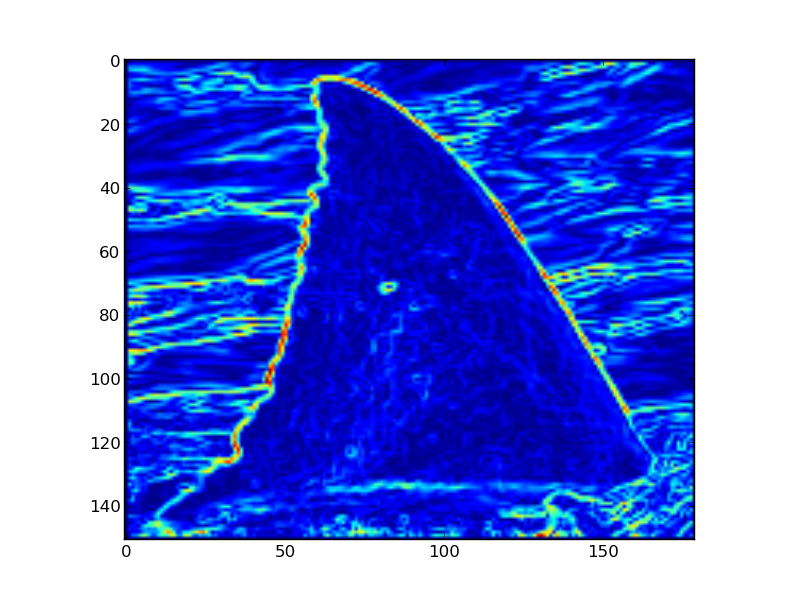
\includegraphics[width=2.5in, height=2in]{haais}
 \caption{A sobel filter applied to a shark fin image}
 \label{fin1}
\end{figure}

\newpage
\noindent Here is a comparison between the effect of the original algorithm on one of the shark fin images and the effect of the modified version of the algorithm on the same image.
\begin{figure}[H]
 \centering
 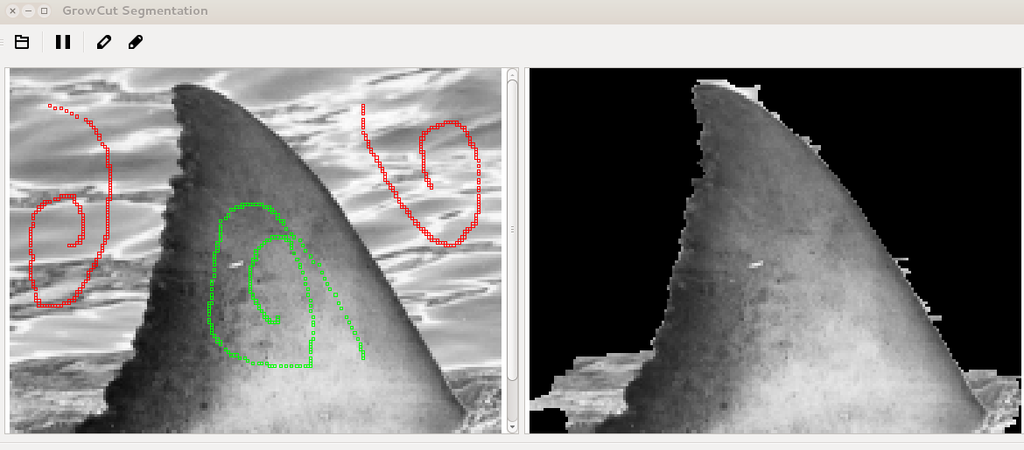
\includegraphics[width=4in, height=1.8in]{haaio}
 \caption{The effect of the original algorithm}
 \label{fin1}
\end{figure}

\begin{figure}[H]
 \centering
 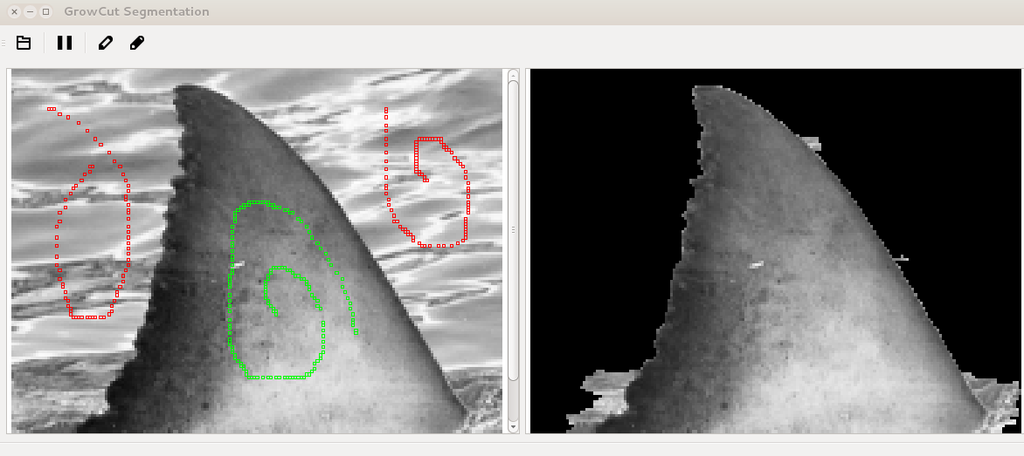
\includegraphics[width=4in, height=1.8in]{haaim}
 \caption{The effect of the modified algorithm}
 \label{fin}
\end{figure}

\noindent It can clearly be seen that the modified version gives better results around the edges, which is essential in the case of the shark fin images.  

\section{Plan for the next two weeks}
The plan for the next two weeks is to optimize the algorithm further to make it effective, not only on the shark fin images but also on a wide variety of images.  
At this stage the algorithm can only work with gray scale images.  This is a definite feature 
which will be studied and updated.  Another feature which will be attempted is to improve the way the algorithm handles edges.  
The goal is to better the algorithm in such a way that it can be included in the Scikit-Image package.  There is also contact with the author of the Grow Cut algorithm(Python)
and he is very excited to hear about our ideas.

\newpage
\bibliography{pr2}

\end{document}

